\section{Containerization}
\label{sec:containerization}
Recalling the Modularity (M) requirement, suppose that a software module requires external dependencies, \emph{e.g.}, libraries or tools to be built and run. These external dependencies may not be made part of the module sources but have to be set up in the systems that host it. Setting up a development and execution environment addressing situations like this is a common but usually also quite complex task. Multiplying the complexities by the number of different hardware platforms that the software module has to run on, one may get a set of problems that are hard to manage. This is the motivation of the Abstraction (A) requirement: the architecture should provide a way to abstract the software modules from the hardware platforms they run on, to allow one to develop software that is portable across different platforms and to simplify the setup of the development and execution environments. Historically, the technology that allowed this kind of abstraction is called \emph{virtualization}, which in general comes at the price of a significant overhead in terms of computational resources and performance. Preventing this is the reason why, in \Cref{sec:prb_requirements}, the Overhead (O) requirement is also stated, which requires the architecture to be as lightweight as possible to avoid any unnecessary computational overheads that may affect the performance of the software modules. The technology that addresses all these requirements, forming a base layer of the proposed architecture, is called \emph{containerization}.

Containerization represents a transformative approach to software deployment that addresses fundamental challenges in application portability and environmental consistency \cite{pahl_cloud_2019}, while remaining distinct from traditional virtualization technologies \cite{dua_virtualization_2014}. While virtualization employs hypervisors to create virtual machines with independent operating systems, containerization achieves isolation by leveraging the host operating system kernel to establish separate environments that share the underlying OS. This architectural difference results in containers exhibiting substantially lower overhead compared to virtual machines, enabling higher resource density and improved efficiency. The technology effectively resolves the challenges of inconsistent behavior across deployment environments by bundling applications with their dependencies, ensuring uniform operation across diverse platforms. This capability proves particularly valuable in distributed software architectures where deployment consistency and scalability are crucial for operational success, while the reduced resource overhead makes containerization an optimal choice for scenarios requiring isolated environments without necessitating complete operating system separation.

The origins of containerization can be traced back to early innovations in Unix-like operating systems. In the early 2000s, technologies such as FreeBSD Jails (2000) and Solaris Containers (2004) introduced the concept of partitioning a single operating system's resources into distinct, isolated instances. FreeBSD Jails enabled administrators to create secure, isolated environments capable of independently running services, while Solaris Containers provided an integrated method for managing multiple isolated application environments on a single instance of Solaris. Concurrently, the Linux ecosystem began to develop foundational features that later form the bedrock of modern containerization technologies. Notably, Linux introduced kernel features such as cgroups (control groups) and namespaces—both essential to containerization's core principles of isolation and resource control. Linux namespaces provide process isolation, determining the visibility of system components like the filesystem, network interfaces, and other processes. In parallel, cgroups regulate the allocation of hardware resources—such as CPU, memory, and I/O—ensuring that containers do not monopolize or starve system resources, thus enabling fair resource sharing and predictable performance.

These features enabled the creation of isolated environments while maintaining efficient resource sharing, ultimately leading to the development of contemporary \emph{container engines}. The efficiency of containerization manifests in reduced overhead compared to virtual machines, as containers eliminate the need for multiple operating systems. This characteristic makes containers particularly suitable for microservices architectures, where applications are decomposed into independently deployable components. The container architecture ensures consistent operation across different infrastructure configurations while allowing potentially conflicting dependencies to coexist without interference.

The operational distinctions between virtualization and containerization significantly influence their respective application domains. Virtualization maintains relevance in scenarios requiring complete operating system isolation, particularly in multi-tenant environments where security and compliance demands necessitate strict workload separation. However, in contexts where such comprehensive isolation proves unnecessary, containerization offers notable advantages in scalability, deployment speed, and resource efficiency. The lightweight nature of containers facilitates rapid provisioning and horizontal scaling, making them particularly advantageous for cloud-native applications and environments requiring dynamic resource allocation.

In the context of this work, containerization can effectively help to build a common architectural ground that abstracts the software modules from the platforms they run on, at the same time packaging with them every external and third-party dependency they require to be built and run. This way, the software modules can be developed and tested in a controlled environment, and then deployed on any platform that supports the containerization technology, a condition that is not restrictive since today container engines are supported on nearly every commercial platform that the proposed solution may target. For this reason, modules and projects based on the proposed architecture are managed through containers: the technical details of this process are postponed to the next chapters, where the architecture is described in detail. To conclude this dissertation, the chosen containerization technology is illustrated in the following section.

\subsection{Docker Engine}
\label{sec:docker}
The release of Docker \cite{docker_inc_docker_nodate} in 2013 was a watershed moment in the evolution and widespread adoption of containerization \cite{merkel_docker_2014,turnbull_docker_2014}. Docker unified the previously fragmented ecosystem of container technologies, incorporating existing Linux kernel features into a cohesive, user-friendly tool that simplified the process of container creation, deployment, and management. Docker's innovation lays in its ability to abstract the underlying complexity of containerization, providing a standardized interface and image format that made the technology accessible to a broader audience of developers and IT professionals. This accessibility facilitated a shift in how software is developed, tested, and deployed.
\begin{figure}[!t]
  \centering
  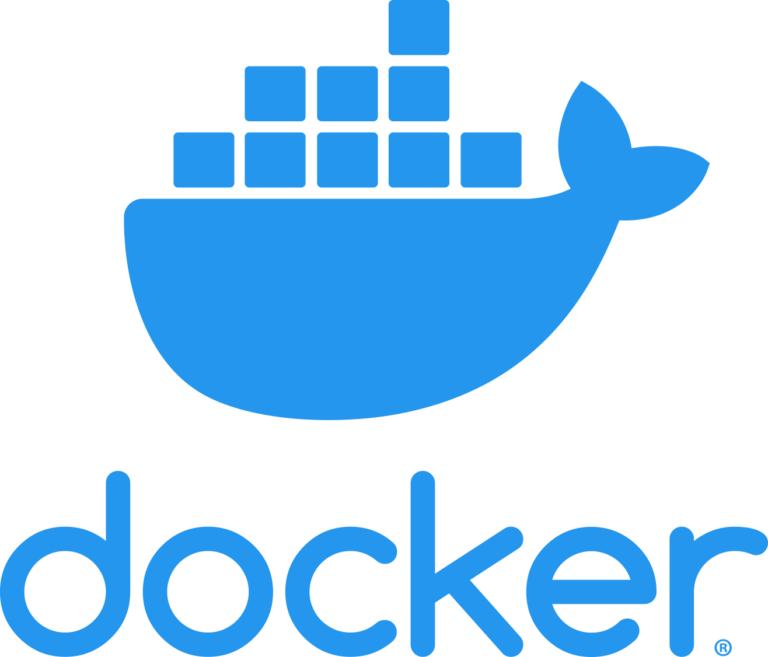
\includegraphics[width=.3\linewidth]{images/ch3/docker.png}
  \caption{Docker logo \cite{docker_inc_docker_nodate}.}
  \label{fig:dockerlogo}
\end{figure}

Docker Hub \cite{docker_inc_docker_nodate-1}, an associated public \emph{registry} of container \emph{images}, further accelerated adoption by providing a central repository from which developers share and reuse container images, promoting community collaboration and reducing redundancy. Moreover, since its birth as a Linux-only tool, Docker has evolved to support also the Windows and macOS operating systems through its Docker Desktop release \cite{docker_inc_docker_nodate-2}, although with a limited set of features available on these platforms, which also require a thin virtualization layer to work. This revolution has also impacted the research world outside of the cloud computing and software development industries, as it has been adopted in many scientific fields to manage the software tools and libraries that are used to analyze data and run simulations, as well as to distribute the results of the research and novel algorithms and procedures in a way that ensures reproducibility, transparency, and accessibility \cite{boettiger_introduction_2015}.

The first key component of Docker's utility is the Dockerfile, which serves as the blueprint for creating Docker images. A Dockerfile is a simple text file that contains a series of instructions on how to assemble a particular Docker image. These instructions include the base image to use, any software dependencies to be installed, environment variables, and commands to be executed when building the image. When a Dockerfile is processed by the Docker engine, it creates a Docker image, which is a read-only template containing the application and its environment. Docker images can then be instantiated as running containers.

Another fundamental feature of Docker is its use of union filesystems \cite{dua_performance_2016}, which are specialized filesystems that merge multiple layers into a single coherent view. Union filesystems are particularly useful in containerization as they allow multiple layers to be stacked, where each layer represents a set of \emph{filesystem changes}. This approach enables efficient storage as new layers can be added or modified without altering the underlying base layers, thereby saving storage space and allowing for rapid image creation and reuse. Specifically, Docker employs OverlayFS by default to create image layers \cite{mizusawa_performance_2017}. Docker images are built in layers, with each layer representing a set of filesystem changes such as installing a package or adding a configuration file. The union filesystem allows Docker to stack these layers on top of each other, presenting them as a single coherent filesystem. This approach provides significant efficiencies in both storage and resource usage, as multiple images can share the same underlying layers. For example, if multiple images are based on the same base operating system image, Docker stores only one copy of that base layer. OverlayFS, for example, enables efficient management of these layers by allowing new changes to be made in an uppermost layer without altering the lower layers, enforcing a copy-on-write mechanism (a paradigm according to which stored data is shared among multiple entities keeping a single copy, until one of such entities has to modify it). This layered approach not only saves disk space but also accelerates the building of new images by reusing existing layers.

Docker Compose \cite{docker_inc_docker_nodate-3} is another powerful tool within the Docker ecosystem that facilitates the management of multi-container applications. With Docker Compose, developers can define and run multi-container Docker applications using a YAML file (Yet Another Markup Language, a popular markup language for configuration and text files) to configure the services, networks, and volumes required by the application. This capability is particularly useful for orchestrating the deployment of complex applications that require multiple components—such as databases, backend services, and front-end web servers—to work together seamlessly. Docker Compose allows these components to be defined as individual services, each in its own container, and specifies how they interact. This simplifies the process of setting up development environments and ensures that the entire application stack can be easily replicated and deployed.

Another crucial feature of Docker are \emph{volumes} and \emph{volume mounts}, which are of paramount importance for data persistence. Containers are ephemeral by nature: when a container is stopped or deleted, all data within it is lost. To overcome this limitation, Docker uses volumes, which are directories or files stored outside the container's writable layer. Volumes can be mounted into one or more containers, allowing data to persist even if a container is removed or updated. This capability is essential for stateful applications, such as databases, which require durable storage that outlives the individual container instances. By using volume mounts, developers can also share data between containers, enabling efficient communication and data exchange between different parts of an application or of a distributed software architecture.

Networking is another key area where Docker provides significant capabilities, enabling containers to communicate with each other and with the outside world. The networking model of Docker includes several types of networks hereby only simply mentioned such as \emph{bridge}, \emph{host}, and \emph{overlay}, each suited to different use cases. Bridge networks are the default and are typically used to enable communication between containers running on the same host. Host networking, on the other hand, allows a container to share the network stack of the host, providing greater network performance and simplifying access to services running on the host. This mode is particularly useful in scenarios where the containerized service needs to avoid the overhead of NAT (Network Address Translation) and requires direct access to the network interfaces available on the host.

Docker also provides mechanisms to control the resources allocated to containers, such as CPU and RAM using, \emph{e.g.}, cgroups on Linux. Resource limiting is critical to ensure that no single container can consume disproportionate system resources, which negatively affects other containers running on the same host. Docker allows users to specify limits on the CPU shares and memory usage for each container, ensuring predictable performance and efficient utilization of system resources. By configuring these limits, administrators can create a balanced environment where all containers receive their fair share of resources, preventing resource contention and ensuring stable operation.

Finally, Docker can use the Linux capabilities subsystem to manage hardware and system call access in a granular manner. Instead of giving containers full root privileges, which poses security risks, Docker allows specific capabilities to be granted as needed. For instance, a container may need the capability to bind to low-numbered network ports or change the system time but it does not need broader privileges that further compromise the host. By selectively enabling only the necessary capabilities, Docker minimizes the attack surface of containers, enhancing security while maintaining the required functionality for each application.

This section presented and described the Docker Engine containerization solution alongside many of its features. The choice of the functionalities to discuss here was not coincidental: each of the features described is essential to the architecture and to fully employ Docker as the solution that addresses the Abstraction (A) requirement. Thanks to the features outlined so far, applications that run inside Docker containers may do so within a simple partition of the host operating system, thus with no additional overhead with respect to, \emph{e.g.}, applications that run on the same system but outside containers. Some configuration on the host is required to achieve this, as the next chapters illustrate, but once everything works this constitutes also a solution to the Overhead (O) requirement. The Docker Engine is used in this work to build and manage hardware and system abstraction layers that establish a common environment for both the development and the execution of software modules and projects among many different platforms.
